\section{Design}
\label{sec:intra-server}

\subsection{Architecture}
\label{subsec:architecture}

\begin{figure*}[t!]
	\centering
	\begin{minipage}{.44\textwidth}
		\centering
		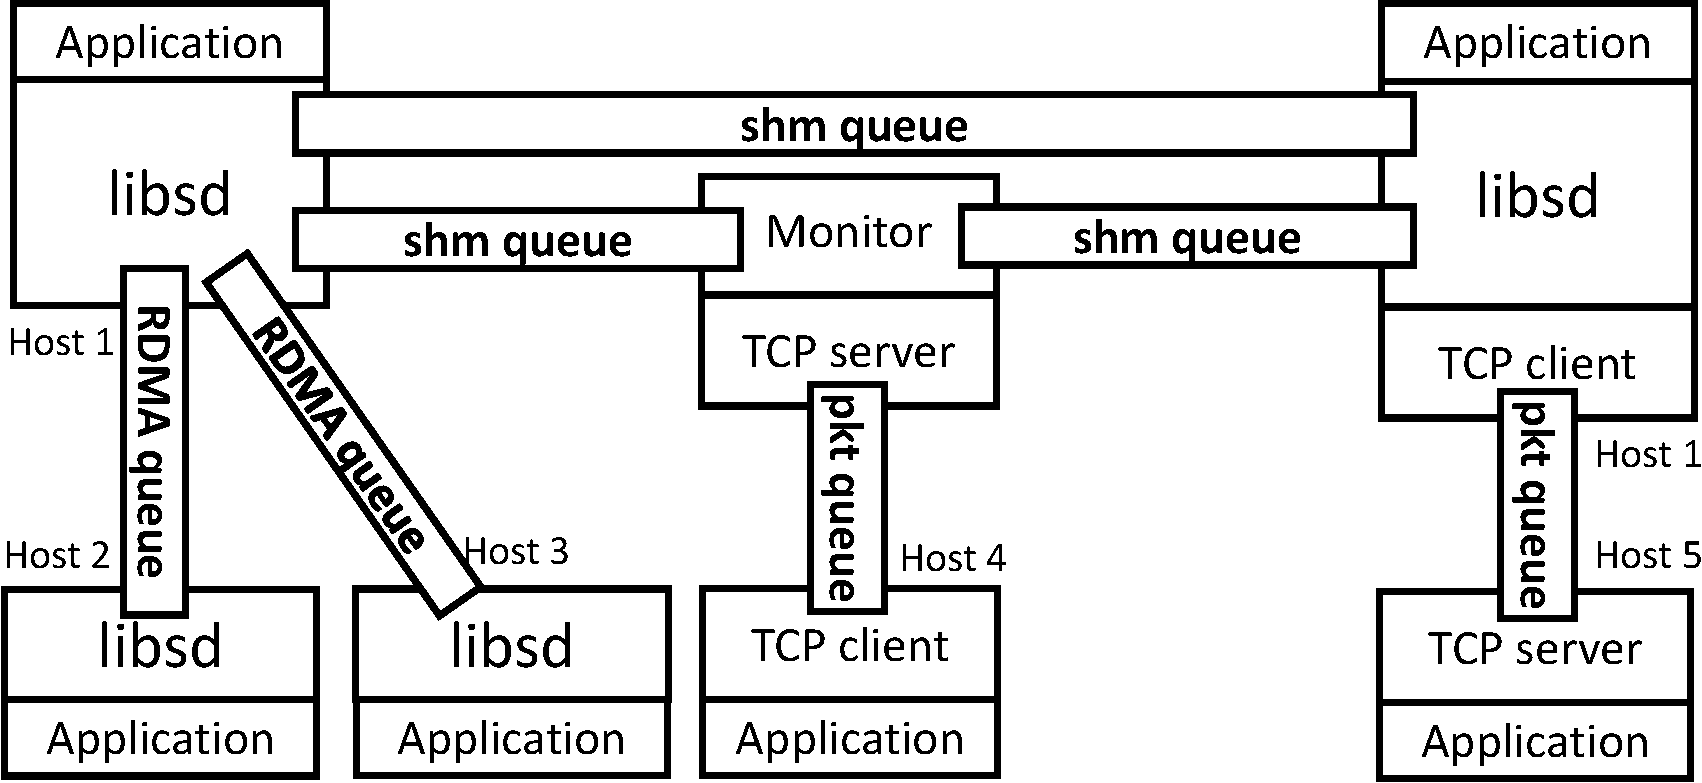
\includegraphics[width=\textwidth]{images/architecture_new}
		\vspace{-5pt}
		\caption{Architecture of \sys{}. Host 1 and 2 are RDMA capable, while host 3 is a regular TCP/IP host.}
		\label{fig:architecture}
		\vspace{-15pt}
	\end{minipage}
	\begin{minipage}{0.3\textwidth}
		\centering
		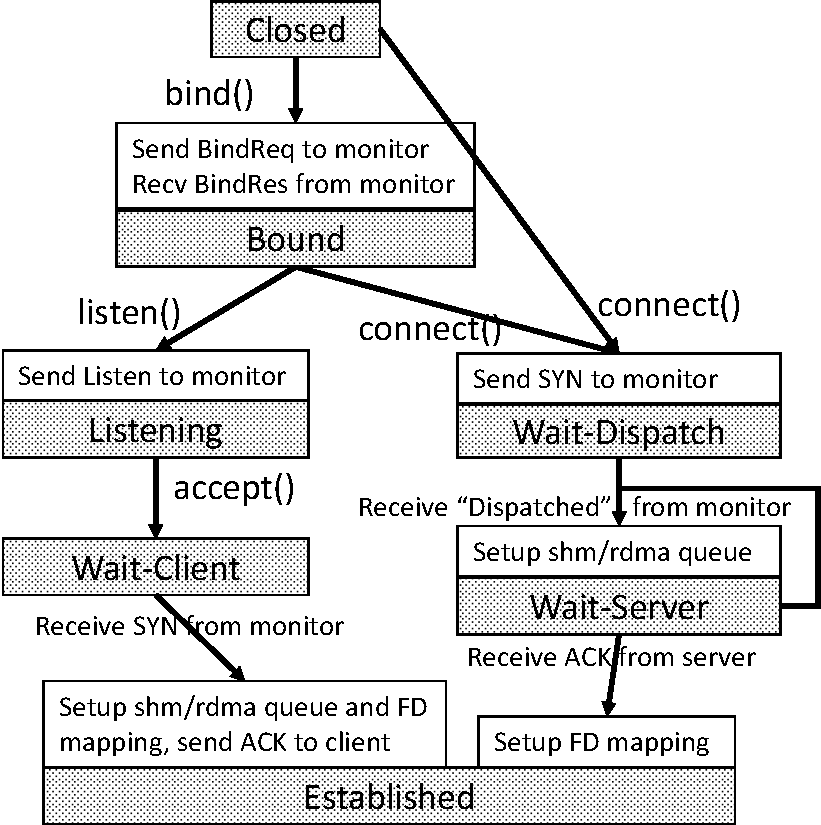
\includegraphics[width=\textwidth]{images/conn-setup-new}
		\caption{State machine of connection creation.}
		\vspace{-5pt}
		\label{fig:conn-setup}
		\vspace{-15pt}
	\end{minipage}
	\begin{minipage}{0.24\textwidth}
		\centering
		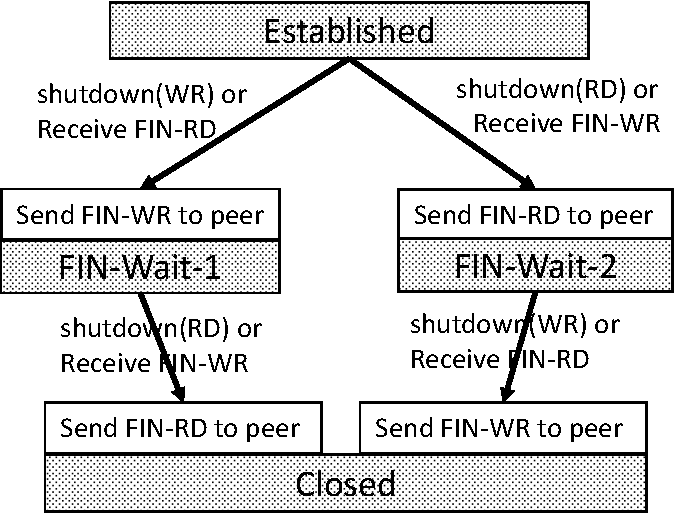
\includegraphics[width=\textwidth]{images/conn-close-new}
		\caption{State machine of connection close.}
		\vspace{-5pt}
		\label{fig:conn-close}
		\vspace{-15pt}
	\end{minipage}
\end{figure*}


As shown in Figure~\ref{fig:architecture}, ...


%Inspired by Unikernels~\cite{madhavapeddy2013unikernels}, we move networking and IPC functions from the kernel to user space. Similar to existing works~\cite{peter2016arrakis,jeong2014mtcp,libvma}, we leverage multiple queues in modern NICs to enable user-space direct access to network. %The kernel is still responsible for process creation, scheduling, virtual memory and device management, but no longer on the critical path of performance.
%To maintain compatibility with existing Linux applications, we design a user-mode library \libipc as a drop-in replacement of the system call wrappers in the GNU C library (glibc). \libipc{} implements network socket functions in user mode, and adds a wrapper to other system calls to track process creation and memory allocation. \libipc{} is not considered a secure domain, as it shares memory space with the application. When \libipc{} is loaded, it creates a Linux native \textit{bootstrap socket} to the \textit{monitor} daemon, then creates a shared memory queue to the monitor.

%Even though multiple threads in the same process share memory space, we still treat each thread as a separated process and use thread-specific storage to store states in \libipc. In the following text, unless explicitly mentioned, we use a ``process'' to refer to a regular process or a thread.

\subsection{Connection Management}
\label{subsec:socket-api}


\parab{Connection creation.}
 in Figure~\ref{fig:conn-setup}...

Client application sends a request to client monitor.
Monitor translates IP addresses (NAT), and forward the request to server application:
If the server application is in the same host, forward the command to server application.
If the client and server applications are in different hosts:
If client monitor has connected to server monitor, forward the request to server monitor.
Otherwise, the client monitor and server monitor establish an RDMA connection (details in next slide).
The server monitor forwards the command to server application.
If the client application has not connected to the server application, the server monitor helps the client and server establish a direct connection.
For intra-host, the monitor allocates a shared memory and sends the shared memory key to both client and server applications.
For inter-host, the client and server monitors proxy information between client and server applications during RDMA setup.
The server application sends a response to client application containing FD mapping. The server application can start sending data immediately after sending the response.
When the client application receives the response, it can start sending data.


\parab{Connection close.} in Figure~\ref{fig:conn-close}...

\parab{Detect whether the peer supports \sys{}.}
Goals: Both client and server can detect whether the peer supports SocksDirect. Use kernel TCP when the peer does not support SocksDirect. No change to kernel.
Server monitor opens a raw socket with libpcap to capture SYN packets to listening ports.
Client monitor opens a raw socket with libpcap to send TCP SYN with a special TCP option, then wait for SYN+ACK response.
If server monitor receives a TCP SYN with special option, respond SYN+ACK with special option and begin SocksDirect establishment.
If client monitor receives a TCP SYN+ACK with special option, the peer supports SocksDirect.
To avoid the kernel TCP stack from sending RST packets, install firewall rules to block incoming SYN and outgoing RST.
If the peer does not support SocksDirect:
The monitor creates a kernel TCP connection using TCP restore functionality.
If the application is able to share network namespace with the monitor, send the restored TCP connection to the application via “sendmsg”. Then the application can use the kernel TCP socket.
Otherwise, the monitor proxies messages between the application and kernel TCP socket.


\textbf{Above is draft.}

\parab{\texttt{Socket}.}
To create a socket connection, an application first calls \texttt{socket} to get a \textit{file descriptor} (FD). 
%Although Linux globally allocates the lowest available file descriptor, this property is rarely used~\cite{han2012megapipe,huang2017high}. We relax the semantics and maintains an FD table in each process. 
We maintains an FD table for each process. Upon allocation, \libipc{} finds an idle FD from the table or doubles the table size if none available. 
%The table is a vector of socket information with an allocation pointer, indexed by FD. Upon allocation, \libipc{} linearly moves the allocation pointer and finds the first idle FD. When the vector is more than half full, its size is doubled. This allows amortized O(1) allocation and O(1) lookup and deletion.
For multi-thread applications, since the FD namespace is shared, we partition the FD namespace to multiple ranges and each thread allocates FD in its range.
%Because per-FD information is local to a process, APIs on socket options are also local.
Because applications still need to access FDs in the kernel (\textit{e.g.} files and devices), we partition the FD space. The kernel assigns FD from zero up to $2^{30}-1$, while \libipc assigns FD from $2^{31}-1$ down to $2^{30}$.

\parab{\texttt{Bind} and \texttt{listen}.}
A \emph{server} process \texttt{bind}s a socket and needs to detect IP and port conflict. In this case, \texttt{bind} is non-partitionable and goes to the monitor. The monitor also listens on the IP and port in a user-space TCP/IP stack (\textit{e.g.} mTCP~\cite{jeong2014mtcp}, LibVMA~\cite{libvma} or Seastar~\cite{seastar}) to receive connections from other hosts.

A \emph{client} process typically \texttt{bind}s without specifying IP and port, so we need to allocate a unique IP and port for it. For scalability, we partition the loopback IP address space (127.0.0.0/8) and each process allocates IP and port in its range.

\parab{\texttt{Connect} and \texttt{accept}.}
When a client process connects to a server process on the same host, it sends a \textit{connect request} to the monitor via shared memory queue. When the server process is on another host, it creates a \textit{bootstrap TCP socket} with a special option via the user-space TCP/IP stack. If the server host supports the option, it is a \sys host and its monitor establishes an RDMA connection to the client to speedup later communications. Otherwise, the client process keeps using the bootstrap TCP socket for compatibility.

On a server host, the monitor distributes connect requests to server processes in a round-robin order, and a \textit{backlog} is maintained in each process. If the client is TCP only, the monitor proxies messages between the server process and the user-space TCP/IP stack. If the client is intra-server or RDMA capable, and it is the first time for the client and server processes to communicate, the monitor creates an inter-process queue for the process pair and sends the credentials to both processes via bootstrap sockets. After a server process \texttt{accept}s a connection in the backlog, it sends a message to the client via inter-process queue to create an FD mapping, then the socket is ready for data transmission. As Figure~\ref{fig:conn-setup} shows, connection creation takes three inter-process delays.

Distributing connection to listeners may lead to starvation when a listener does not \texttt{accept} new connections. We devise a \textit{work stealing} approach. When a listener \texttt{accept}s from empty backlog, it requests the monitor to steal from others' backlog. To avoid polling empty backlogs, each listener notifies the monitor when its backlog becomes empty. To avoid contention between a listener and monitor, the monitor sends a request to the listener rather than stealing from the backlog directly.

%\subsubsection{Connection Close}

\parab{\texttt{Close} and \texttt{shutdown}.}
Connection close is a peer-to-peer operation because only the peer process needs to be notified. If FD is deleted immediately after \texttt{close}, a new connection may reuse the FD while the peer process might not yet have received the close event thus sends data to the wrong connection. To avoid this, we require a handshake between peers.
Because socket is bidirectional, \texttt{close} is equivalent to \texttt{shutdown} on both send and receive directions.
When application shuts down one direction of a connection, it sends a \textit{shutdown message} to the peer. The peer responds with a shutdown message. A process deletes an FD when it receives shutdown messages in both directions.

%In order to achieve high scalability, we separate scalable operations to different processes. To avoid the overhead of contention, \libipc enable the file descriptor allocation by individual process and when a connection is setup, the other peer of the connection gets notified of the file descriptor number by message passing. Since we treat different threads in one process as different processes, we allocate file descriptor of different ranges to each of them to avoid collision. Since file descriptor is managed separately by each process, it is possible that a file descriptor is reused after the connection is closed. Our solution is that resources of a file descriptor is not released until an ACK is received for the close operation.

%Generally, each process in our design is treated as an endpoint in the network. Figure \ref{fig:conn-setup-close} shows the process of connection setup and close. When \textit{socket} is called, the process itself allocate per fd resources. When \textit{listen} is called, monitor is notified of port occupation. During the \textit{connect} operation, monitor first chooses one of the processes listen on this port then coordinates the creation of the shared memory between the two processes and notifies each other of the new connection. When \textit{close} happens, both of the endpoint notify each other and monitor is responsible to destroy the shared memory between them. 







\subsection{Sharing a Socket Among Processes}
\label{subsec:fork}
Process fork and thread creation are ubiquitous in modern applications. 
Fork and thread makes sockets to be shared, and thus become a multiple producers or multiple consumers model. With a traditional mutual exclusion solution, the multi-process scalability of socket is limited. Our aim is to maximize the common-case performance while keeping compatibility with Linux socket.

We make two observations: First, fork and thread creation are not frequent in high performance applications compared to connection setup and data transmission.
Second, it is uncommon that several processes \texttt{recv} concurrently from a shared socket, because the streaming semantics of socket makes it hard to avoid receiving incomplete messages. 
%For such producer-consumer scenarios, message brokers~\cite{hintjens2013zeromq,rabbitmq2017rabbitmq,kreps2011kafka} are typically used.
Based on the observations, we propose the following requirements:

\begin{enumerate}[noitemsep,nolistsep]
 \item \textbf{Synchronization-free.} With multiple potential senders and receivers, if only one pair of sender and receiver is active, the throughput and latency should be comparable with that of a sender-receiver pair.
 \item \textbf{Multi-sender scalability.} Multiple processes may send data concurrently through a shared socket. With multiple active senders and a single receiver, if the receiver is not a bottleneck, the throughput should scale.
 \item \textbf{Self-stabilization.} Certain operations (\textit{e.g.} \texttt{fork}) may slow down the system temporarily, but after that the throughput should converge back to normal.
\end{enumerate}

For compatibility with Linux semantics, we also need to ensure message ordering and liveness:
\begin{enumerate}[noitemsep,nolistsep]
\item \textbf{Single receiver ordering.} For a specific pair of sender and receiver, the received messages have the same ordering as they were sent.
\item \textbf{Multiple receiver ordering.} The order of \texttt{send} and \texttt{recv} operations for one sender and multiple receivers should be linearizable. If receiver $R_1$ already receives $D_1$, then receiver $R_2$ calls \texttt{recv} and gets $D_2$, we guarantee that $D_1$ is sent before $D_2$.
\item \textbf{Deadlock-free.} If a socket buffer is not empty when \texttt{recv} is called by one or more receivers, at least one receiver should get data.
\item \textbf{Starvation-free.} If a sender keeps sending, any receiver trying to \texttt{recv} will eventually get data.
\end{enumerate}

Our scalable socket design can be divided into four parts: a) \texttt{send} and \texttt{recv}, b) adding new senders and receivers (\texttt{fork} and \texttt{pthread\_create}), c) connection creation and d) connection close.

\subsubsection{Send/Recv Operation}
\label{subsubsec:fork_rdwr}
\begin{figure}[t]
	\centering
	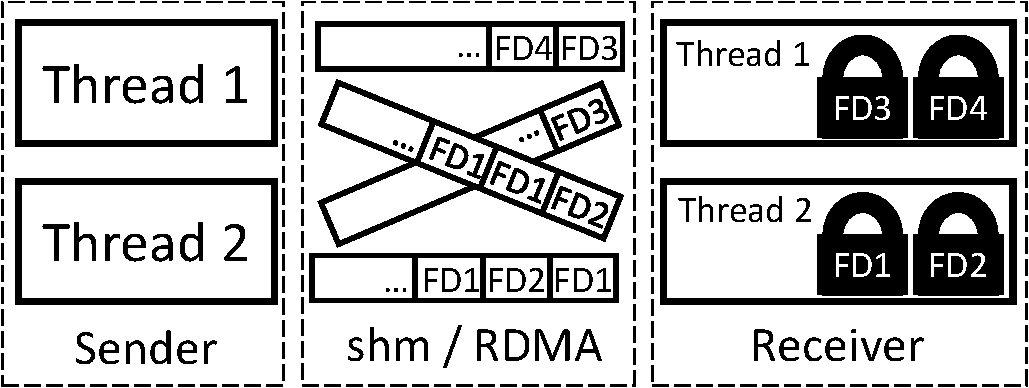
\includegraphics[width=0.3\textwidth]{images/fork_rdwr}
	\caption{Two senders and two receivers share a socket. Receiver 2 is designated by both senders.}
	\label{fig:fork-rdwr}
	\vspace{-15pt}
\end{figure}
In this section, we assume that a socket is connected and the number of senders and receivers are constant.

\parab{Multiple concurrent senders.}
In order to avoid synchronization, we create queues between \emph{every} pair of senders and receivers, as Figure~\ref{fig:fork-rdwr} shows. %The queues form a bipartite graph between senders and receivers. 
Each receiver polls messages from all sender queues in round-robin order. Therefore, the multi-sender throughput can scale.
%Figure \ref{fig:fork-bipartitegraph} shows a sample of the shared-memory buffers between senders and receivers for one connection.

\parab{One exclusive receiver.}
Each sender, though has a queue to every receiver, designates only a single receiver with exclusive access to the socket and only send data through the corresponding queue. 
In the common cases with only a single active receiver, the performance would be the same as one-to-one communication. 
%It is challenging for the sender to choose a receiver, since the chosen one may not call \texttt{recv}, while other receivers may be under starvation. 

\parab{Switch to a receiver.}
When a non-designated receiver attempts to \texttt{recv} from the socket, it sends a \textit{takeover request} to the sender. 
Up receiving the request, the sender %processes takeover requests in FIFO order to avoid starvation and 
designate the requester as the new exclusive receiver and remove the status from the old designated receiver. 
%Another challenge is that when a receiver should send a takeover request. 
%Each receiver maintains a flag locally to indicate whether it is designated by the sender. The flag is flipped when the receiver gets takeover request or completion from sender. When a receiver tries to \texttt{recv} and finds itself not designated, it sends a takeover request to sender. Before the receiver becomes designated, the takeover request is sent only once.

\parab{Remaining data in queue.}
A challenge arise when there is remaining data in the queue when a receiver requests to take over the socket. %We need to ensure that all the remaining data can be received by the new receiver. 
%Because multiple sockets share a queue from sender to each receiver, and different sockets have different designated receivers, the new receiver cannot access the queue from the old receiver directly. Instead, 
The remaining data needs to migrate from the old active queue to the new active queue. When the sender processes a takeover request, it first forwards it to the current receiver. Upon receiving takeover request, the current receiver returns all remaining data to sender via \textit{takeover completion} messages, which the sender forwards to the new receiver. During migration, the sender blocks \texttt{send} operations and takeover requests to ensure message ordering.


%\begin{figure}[t]
%	\centering
%	
\includegraphics[width=0.3\textwidth]{images/fixme}
%	\caption{This figure shows a stable connection handled by multiple senders and receivers.}
%	\label{fig:fork-bipartitegraph}
%\end{figure}

\subsubsection{Fork and Thread Creation}
\label{subsubsec:fork_fork}


\begin{figure}[t]
	\centering
	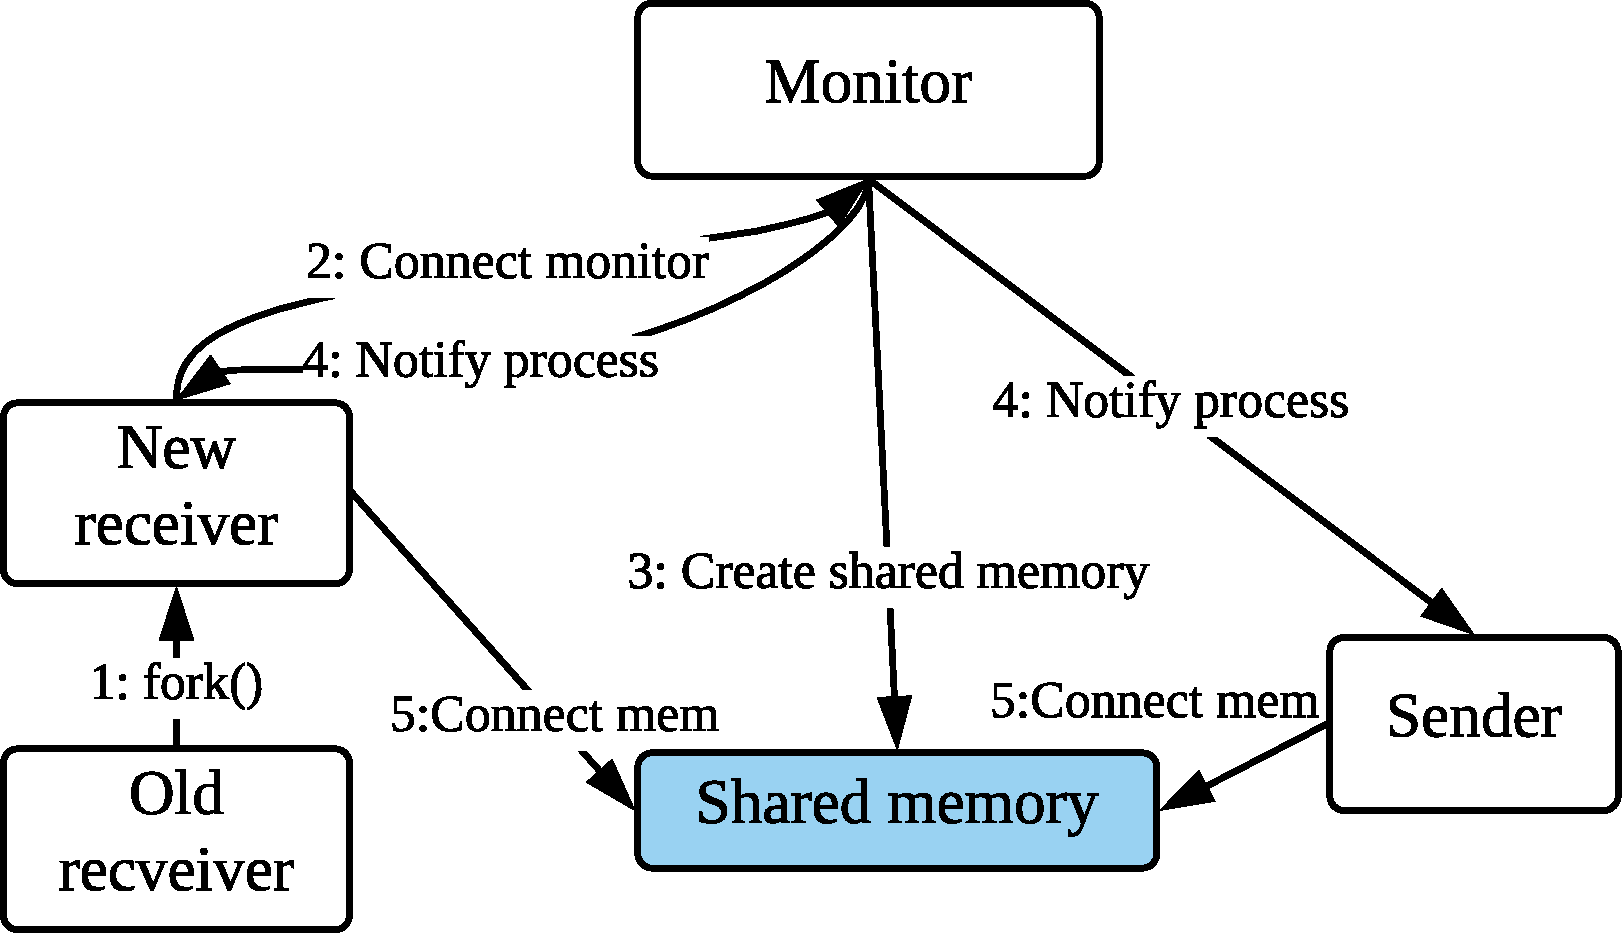
\includegraphics[width=0.4\textwidth]{images/fork}
	\caption{Message flow during \texttt{fork}.}
	\label{fig:fork-fork}
	\vspace{-15pt}
\end{figure}


The first challenge with fork and thread creation is how to identify and isolate parent and child processes. As shown in Figure~\ref{fig:fork-fork}, when the application calls \texttt{fork}, \texttt{clone} or \texttt{pthread\_create}, \libipc{} first generates a secret for pairing, then invokes the corresponding system call. After fork, parent and child independently creates a \textit{bootstrap socket} to the monitor and sends the secret (child inherits parent memory space and knows the secret). The monitor can thus pairs the child process with the parent. 
To maintain isolation between parent and child, monitor creates new shared memory queues to replace all queues in \emph{both} parent and child. We do not reuse queues due to potential isolation violation. %The monitor then sends credentials of new queues to parent and child via bootstrap sockets. 
Each peer process is also notified of the new queues and the new process. From then on, parent and child processes have isolated queues to the monitor and peers.

%A harder challenge comes from socket connection sharing between parent and child processes. 
Upon fork, each connection needs to add a sender to the sending direction and a receiver to the receiving direction. A major challenge is how to handle the remaining data in the original send and receive queues.

%For each unidirectional queue, we discuss the behavior of related processes in four cases:
%\begin{enumerate}
%	\item A sender process itself forks.
%	\item A receiver of a sender process forks.
%	\item A receiver process itself forks.
%	\item A sender of a receiver process forks.
%\end{enumerate}

%The general process of fork is that after monitor is notified of the fork, it creates shared memory between the newly created process and all the processes which previously have connections with the parent process. The key challenge lies in the fork is that how to deal with the existing data in the connection to guarantee the order requirements.

\parab{Receiver fork.}
First we look at a simple case when a receiver forks. Recall that only one receiver has exclusive access to a socket, as stated in Sec.~\ref{subsubsec:fork_rdwr}. The parent process inherits receive permission. When a sender receives fork notification of its peer, it copies all data from original queues to new queues of the parent process.

\parab{Sender fork.}
When a sender forks, things are more complicated. We need to guarantee that all data sent prior to \texttt{fork} is consumed before the data sent after \texttt{fork}.

Our solution is to let receivers drain the original queue first before switching to the new queues. After \texttt{fork}, both parent and child send data to its new queue. When the receiver is notified of the fork, it keeps track of the original queue and consumes all data in it before activating new queues. Note that the parent or child may fork again before the original queue is drained. With this in mind, the receiver maintains a forest data structure to track dependency of queues. The root of each tree in the forest is the oldest queue to receive from. Each non-leaf node has two children indicating the new queue of parent and child processes. If a non-leaf root queue becomes empty, it will be removed, and the two children queues will be promoted to root nodes.

\parab{Takeover During Fork.}
After a sender forks, the receivers still need the takeover mechanism to arbitrate remaining messages in the original shared memory queue. However, both parent and child senders have dropped the original queue and will not respond to takeover requests. A similar situation occurs when a sender process dies. Our solution is to let the receivers use atomic operations to compete for remaining data in the original queue. Since this case rarely happens, the performance of the overall design is not affected.


%Things become much more complicated when cases 1,4 happens after cases 2,3 happening. After receiver forks, the unique sender is responsible for receiving ``takeover message'' and resend the data to new receivers. However, if sender forks following the receiver forks, according to the methods we mentioned above, there is no sender responsible for processing ``takeover message''. Our solution is that we require the receivers to poll the data from the old shared memory queue and compete for data. Since this case rarely happens, the performance of the overall design is not affected.

\subsubsection{Connection Creation}
\label{subsubsec:fork_new}

%A connection created after \texttt{fork} cannot be accessed by its sibling process, while 
A connection created by a thread can be accessed by all threads in the same process. To minimize state sharing, \libipc assigns a unique file descriptor (FD) space to each thread, so that each thread can allocate FDs locally. 
% and determine which thread a FD belongs to. 
During connection creation, \libipc does not share the FD eagerly with other threads, because most threads in existing applications do not use connections created by other threads.
When a thread do want to accesses a FD that belongs to another thread, \libipc sends a message to the owner thread and requests sharing the FD. This procedure is exactly the same as sharing existing connections during thread creation (Sec.~\ref{subsubsec:fork_fork}). %The sharing procedure only happens once for every connection and thread. Sharing existing connections eagerly during thread creation is an optimization. First, children threads are more likely to use existing connections than siblings. Second, batch processing improves performance.

\subsubsection{Connection Close}
\label{subsubsec:fork_close}

%Close is the operation that all of the processes leave the connection. The synchronization is  especially challenging since all the processes are run in parallel. One challenge lies in file descriptors are managed by decentralized processes and are possibly reused. One process close a connection while the others are doing compute intensive tasks is a case. It is possible that the file descriptor of the old process is reused and a new connection is setup with the same file descriptor. The other process may notice the close of the old connection and also call close on its own side, which lead to the new connection setup by the previous process closed due to the match of same file descriptor. 

%To satisfy the synchronization requirements, the close function call is all completed by message passing. The caller of close need to wait for ACK from all the other peers before release resources. i.e. the status of the connection.

%\parab{Broadcast.}
When a process calls \texttt{close}, all its peers cannot send to or receive from the FD. In this sense, closing a shared connection needs to multicast a notification to the peers and collect responses from them. A challenge arise when \texttt{close} is interleaved with \texttt{fork}. Since \texttt{fork} and \texttt{close} do not commute~\cite{clements2015scalable}, we need a rule to determine their partial order. We make the choice that the ordering is determined by the initiator of \texttt{close}. If a process calls \texttt{close} before receiving fork notification, it will piggyback close notification with fork completion to both parent and child processes.

%\parab{Handshake before releasing resource.}
%Another challenge is caused by FD reuse after close. As stated in Sec.~\ref{subsec:socket-api}, a FD is deleted after receiving shutdown message of both directions. With multiple processes sharing a connection, after one process calls \texttt{close}, others can still use the connection. Consequently, a process deletes a FD only after receiving shutdown messages of both directions from all peers of the FD.

%Another challenge lies in the close of a connection is that close is a broadcast operation while send/receive is sent to a specific process. Besides, fork and close are immutable operations while the scalability requirements of the system impose the constraint that all the operations run asynchronously. As a result, a rule to determine the partial order is required.

%In \libipc, we make the choice that the order of fork and close is determined at the start point of the fork operation and the end point (after receiving all the ACKs). By making this choice, when a process waiting fork close ACK encounters fork message, it could send a separate close request to newly created process, which guarantees all the processes closed.


\subsection{Multiplex Sockets via One Queue}
\label{subsec:multiplex-conn}

To scale the system with multiple cores, each process should be able to transmit data directly to the peer without notifying monitor. As shown in Table~\ref{tab:socket-api}, we design all APIs in data transmission to be peer-to-peer or local.

\parab{Multiplex connections in event-driven applications.}
To reduce memory footprint and improve locality of memory accesses, we use one queue to multiplex all connections between a pair of processes. Each data item in the queue is marked with its FD. By using a single queue, we save per-socket memory footprint, and random memory accesses and cache misses are reduced (See Sec.~\ref{subsec:challenges}). However, head-of-line blocking problem would arise if the queue is FIFO. 
%If we use a FIFO queue, the application would block if it \texttt{recv} from a connection with data not at the head of queue. 
Therefore, the queue needs to support picking a message in the middle with a specific FD. 
Fortunately, this does not happen frequently. Event-driven applications typically process incoming events in a FIFO order. For \texttt{epoll\_wait} in level trigger mode, we iterate through all messages in the queue and return those in the set of registered FDs. When applications call \texttt{recv}, \libipc{} would usually dequeue the message at head.

We maintain a bitmap of the epoll FD set.
When epoll\_wait() is called, we scan all data queues round-robin and check the FD of each data message against the bitmap. If the FD is in the bitmap, an event is returned to the application.
A global cursor is maintained to resume data queue scanning from the last position in the last scanned queue.
A per-queue cursor records the last scanned position in each queue to avoid scanning a message twice.
Each FD maintains the positions of the first and last scanned (but unread) message of the FD.
When a new message of the FD is scanned, a pointer in the last message is updated to point to the new message. This chains received messages of a FD to a linked list.
This is to speedup receive operation. When an application attempts to receive multiple messages from a FD, it can follow the linked list rather than scanning through the whole queue.

%Because both \texttt{epoll\_wait} and \texttt{recv} access a same queue, each data transmission involves only one cache migration.

To poll events from sockets and other FDs (handled by kernel) at the same time, \libipc{} creates an \textit{epoll thread} in each process to wait on all FDs handled by kernel. When it receives a kernel event, it broadcasts the event to application threads via shared memory queues. %\texttt{Epoll\_wait} in \libipc{} will return such kernel events in addition to socket events. %Note that Linux allows an event to be received by multiple threads sharing the FD.

\parab{Head-of-line blocking.}
Head-of-line blocking causes two problems.
First is to receive control messages when the queue is full. For example, in order to close the receive direction while sending data, the shutdown message should not be blocked by unconsumed data in the queue. To transfer control messages out-of-band, we add an \textit{emergency queue} alongside each data queue.
A receiver will always retrieve messages in the emergency queue immediately.

Second, if application does not receive from an FD for a long time, data items of the FD may fill up the queue and starve other FDs.
When data queue is full, the sender sends a message via emergency queue to trigger garbage collection in the receiver.
The receiver scans empty space in the middle of queue and moves messages closer to the tail, so that empty space are collected at the head and can be returned to the sender.
%To avoid starvation, we need at least one byte of headroom per FD. Accordingly, we design a single byte \textit{headroom slot} per FD. When data queue is full and the per-FD headroom slot is free, sender uses it and sends a notification via emergency queue. Receiver receives from data queue first, then from the headroom slot if it received a notification.

